\documentclass[oneside]{article}
\usepackage{hyperref}
\hypersetup{
	colorlinks, 
	citecolor=black,
	filecolor=black,
	linkcolor=black,
	urlcolor=black
}

\usepackage[]{algorithm2e}
\SetKw{Assert}{assert}
\SetKw{Contradiction}{contradiction}
\usepackage{drawstack}

\usepackage[framemethod=tikz]{mdframed}
\mdtheorem[linecolor=blue,frametitlerule=true]{definition}{Definition}
\mdtheorem[linecolor=red,frametitlerule=true]{example}{Example}
\mdtheorem[linecolor=green,frametitlerule=true]{lemma}{Lemma}

\usepackage{marginnote}
\usepackage{geometry}
\usepackage{tikz}
\usepackage[utf8]{inputenc}
\usepackage{listings}
\lstset{tabsize=3}
\definecolor{lightred}{rgb}{1,0.9,0.9}
\lstset{backgroundcolor=\color{lightred}}
%\lstset{numbers=left}


\usepackage{VassorTitle}

\institution{École polytechnique fédérale de Lausanne}
\title{Verified double-hashing hash map}
\supervisor{
	K. \textsc{Argyraki}, Pr.\\
	G. \textsc{Candea}, Pr.\\
	A. \textsc{Zaostrovnykh}, Ph. D. Student
}
\project{Optional Semester Project}
\author{Martin \textsc{Vassor}}
\date{\today}

\newcommand{\keyvalue}[2] {
	\begin{tabular}{| p{0.8cm} | p{1.3cm} |}
			\hline
			\texttt{#1} & \texttt{#2} \\
			\hline
		\end{tabular}
}

\begin{document}
\maketitle

\newgeometry{outer=4.5cm, marginparwidth=3cm, marginparsep=-0.5cm}
\section{Introduction}
This report explains, in an informal way, the implementation and verification of a double-hash hash map. It does not aim to provide a complete and detailed explication of each line of code. Instead, the goal is to synthesize the main points needed to understand both the code and the verification.

The actual verification contains more than 100 new lemmas and fixpoints, and it would make no sense to formally describe each of them here, as formal definitions and proofs are provided. Also, most of those are simple and the name is explicit enough to understand their behaviour.

Thus, this document is more intended to be a companion to understand the actual proof.


\section{Implementation}
\subsection{Provided implementation}
I was provided a naive hash map implementation, in which a $<key, value>$ tuple is inserted at the first free cell after $h(key)$, where $h$ is a given hash function.

Thus, in case of multiple conflicts, the same cells will be tested. For instance, in Example~\ref{expl:naive_impl}, if $h(key1) = h(key2) = h(key3)$, then there is $2$ unsuccessful accesses before finding an empty cell to insert $key3$ in.

\begin{example}[Multiple conflicts when inserting in a naive hash map.]
	\label{expl:naive_impl}
	\begin{center}
		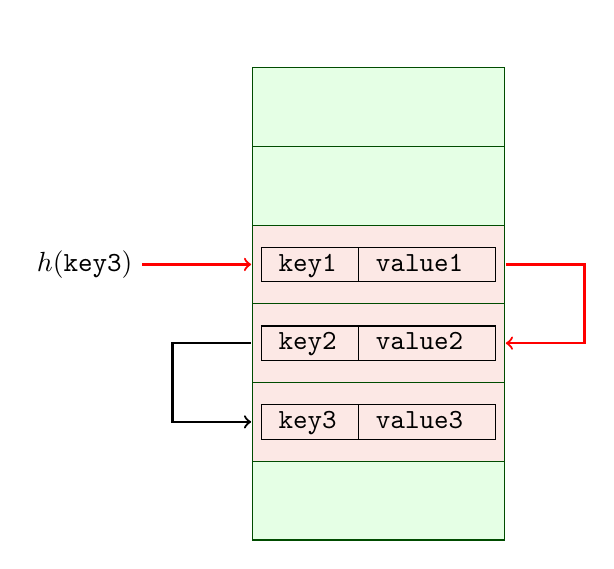
\begin{tikzpicture}
			\draw (0, -3) node[anchor=east] (key3) {$h(\mathtt{key3})$};

			\drawstruct{(3,0)}
			\structcell[freecell]{} \coordinate(firstCell) at (currentcell.east) ;
			\structcell[freecell]{} \coordinate(secondCell) at (currentcell.east);
			\structcell[occupiedcell]{\keyvalue{key1}{value1}} \coordinate(thirdCell) at (currentcell.west); \coordinate(thirdCellOut) at (currentcell.east);
			\structcell[occupiedcell]{\keyvalue{key2}{value2}} \coordinate(fourthCell) at (currentcell.west); \coordinate(fourthCellOut) at (currentcell.east);
			\structcell[occupiedcell]{\keyvalue{key3}{value3}} \coordinate(fifthCell) at (currentcell.west); \coordinate(fifthCellOut) at (currentcell.east);
			\structcell[freecell]{} \coordinate(sixthCell) at (currentcell.east);

			\draw[->, red, thick] (key3) -- (thirdCell);
			\draw[->, red, thick] (thirdCellOut) -- ++(1, 0) |- (fourthCellOut);
			\draw[->, thick] (fourthCell) -- ++(-1, 0) |- (fifthCell);
		\end{tikzpicture}
	\end{center}
\end{example}

\subsection{Double-hash implementation}
The solution implemented during this project is \emph{double-hashing}. In double-hashing, instead of searching in the following cell in case of conflict, the key is re-hashed using a second hash-function. This second hash-function determines an offset, and after each unsuccessful try, the $current\_index + offset$-th cell is looked-up. 

For instance, Example~\ref{expl:double_h_impl} shows the same accesses as the previous example, but with double-hashing (the first hash-function being the same). As $key2$ and $key3$ have different second hashes, their second choice cell is not the same. Then inserting $key3$ only conflicts with $key1$. 

\begin{example}[Multiple conflicts when inserting in a double-hash hash map.]
	\label{expl:double_h_impl}
	\begin{center}
		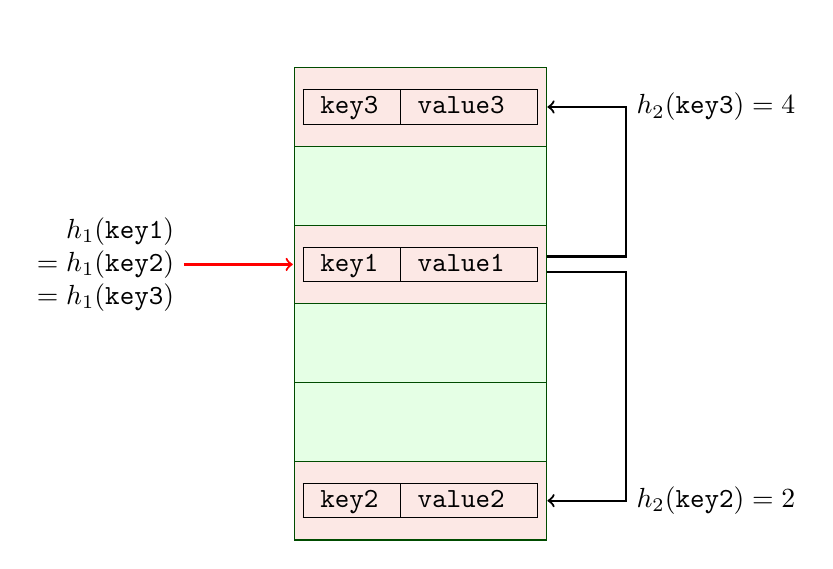
\begin{tikzpicture}
			\draw (0, -3) node[align=right,anchor=east] (key3) {$h_1(\mathtt{key1})$\\$ = h_1(\mathtt{key2})$\\$=h_1(\mathtt{key3})$};

			\drawstruct{(3,0)}
			\structcell[occupiedcell]{\keyvalue{key3}{value3}} \coordinate(firstCell) at (currentcell.east) ; \coordinate(firstCellOut) at (currentcell.east);
			\structcell[freecell]{} \coordinate(secondCell) at (currentcell.east);
			\structcell[occupiedcell]{\keyvalue{key1}{value1}} \coordinate(thirdCell) at (currentcell.west); \coordinate(thirdCellOut) at (currentcell.east);
			\structcell[freecell]{} \coordinate(fourthCell) at (currentcell.east); \coordinate(fourthCellOut) at (currentcell.east);
			\structcell[freecell]{} \coordinate(fifthCell) at (currentcell.west); \coordinate(fifthCellOut) at (currentcell.east);
			\structcell[occupiedcell]{\keyvalue{key2}{value2}} \coordinate(sixthCell) at (currentcell.east); \coordinate(sixthCellOut) at (currentcell.east);

			\draw[->, red, thick] (key3) -- (thirdCell);
			\draw[->, thick] (thirdCellOut) +(0,0.1) -- ++(1, 0.1) |- (firstCellOut) node [pos=0.5, anchor=west] {$h_2(\mathtt{key3})=4$};
			\draw[->, thick] (thirdCellOut) +(0,-0.1)-- ++(1, -0.1) |- (sixthCellOut) node [pos=0.5, anchor=west] {$h_2(\mathtt{key2})=2$};
		\end{tikzpicture}
	\end{center}
\end{example}
\subsection{Benchmark}
We tested two cases: the general case, where any value can be searched for. The worst case been trying to access a value not present (this requires to go through the whole array), we tested a second realistic case, where the values searched for were in the map. 

We compared the results with the naive implementation and with two C++ implementations using the standard \texttt{unordered\_map} data structure. The first C++ version uses the default hash function, the second uses the same hash function as in the C versions.

The test consists of uniformly distributed accesses (among all possible keys in the general case, and among existing keys in the second one). The probability of insertion/deletion is determined in function of the current load and the target load.

The following subsections show the results for both cases, for 70\% of read accesses. It appears that the percentage of read accesses does not influence ``the shape'' of the result. Results for other read proportions, as well as raw data, are available on the github repository.

The code was compiled with GCC 4.9.3. It appears that bug as been reported for version greater than 4.6.2: performances of \texttt{unordered\_map} are $3\times$ slower compared to 4.6.2\footnote{\url{https://gcc.gnu.org/bugzilla/show_bug.cgi?id=54075}}.
\subsubsection{General case}
Figure~\ref{fig:result_contains} present the results, in the general case. For this test case, 10000 accesses were performed. The interesting point is that the double hash implementation perform better with higher loads than with low loads. This behaviour is due to the fact that the probability that a key is present increases with load. Hence, in an execution at higher load, there are less misses than at low loads. 

At low loads, the naive implementation performs better than the double hash one. This is a good illustration of the locality problem: in the naive implementation, accesses are performed in order. Then, both spatial locality of cache lines and address prediction works better. An evaluation with cachegrind shows the difference (see Example~\ref{expl:cache}).
\begin{example}[Cache accesses]
	\label{expl:cache}
Cachegrind results for load = $10\%$, $70\%$ of read accesses, first for the naive implementation: 
	\begin{verbatim}
D   refs:        319,195,365  (297,779,797 rd   + 21,415,568 wr)
D1  misses:       27,235,744  ( 27,203,118 rd   +     32,626 wr)
LLd misses:           10,861  (      5,701 rd   +      5,160 wr)
D1  miss rate:           8.5% (        9.1%     +        0.1%  )
LLd miss rate:           0.0% (        0.0%     +        0.0%  )
	\end{verbatim}
And for the double hash implementation: 
	\begin{verbatim}
D   refs:        328,259,239  (328,032,233 rd   + 227,006 wr)
D1  misses:      303,932,169  (303,902,705 rd   +  29,464 wr)
LLd misses:           11,745  (      4,032 rd   +   7,713 wr)
D1  miss rate:          92.5% (       92.6%     +    12.9%  )
LLd miss rate:           0.0% (        0.0%     +     3.3%  )
	\end{verbatim}

In this example, there are more than $90\%$ of data cache misses in L1 for the double hash implementation, while the naive one achieve less than $10\%$. In the double hash implementation, almost all accesses hit on the LLC.
\end{example}

\begin{figure}
	\centering
	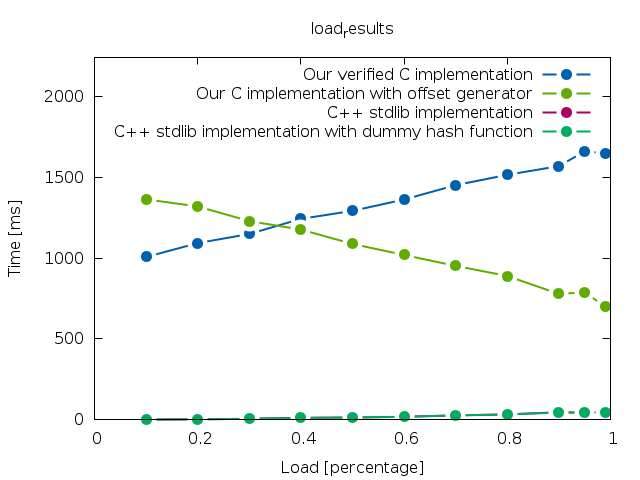
\includegraphics[height=.45\textheight]{result_example_contains.png}
	\caption{Timings for 70\% read accesses, including non existing keys.}
	\label{fig:result_contains}
\end{figure}

\subsubsection{Access only existing keys}
In the case all accessed keys exist, double hash implementation is approximatively an order of magnitude faster than C++, on GCC 4.9.3. However, some performance issues have been reported for \texttt{unordered\_map} higher than 4.7.1 ($3\times$ slower than 4.6.2). Hence, this performance evaluation should be performed again with a lower version for a fair comparison. 

However, compared to the naive C implementation, the results are quite good: the double hash implementation is $2$ orders of magnitude faster than the naive one.

\begin{figure}
	\centering
	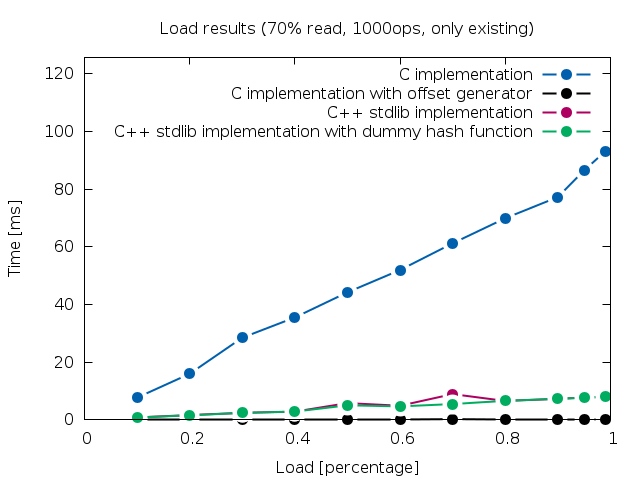
\includegraphics[height=.45\textheight]{result_example_no_contains.png}
	\caption{Timings for 70\% read accesses, excluding non existing keys.}
	\label{fig:result_no_contains}
\end{figure}

\section{Verification}

\subsection{Provided proof}
\subsubsection{Requirement (\texttt{R})}
\marginnote{\texttt{up\_to(nat, prop)} verifies that \texttt{prop} is ensured for all \texttt{i} below \texttt{nat}: \\
\texttt{up\_to(0, prop) = true}\\
\texttt{up\_to(n, prop) = prop(n-1) \&\& up\_to(n-1, prop)}}
Figure~\ref{fig:for_loop_orig_pruned} presents the relevant part of the proof of the original loop in \texttt{find\_key}. The last statement (\texttt{no\_key\_found(ks, k)}) requires the property \texttt{not\_my\_key(k)} to be verified for all current keys in the mapping, ensured by the \texttt{up\_to(nat\_of\_int(length(ks)), \ldots(not\_my\_key)(k)\ldots)} statement.

The \emph{for}-loop invariant proves this \texttt{up\_to} statement: at each round, \texttt{not\_my\_key(k, nth(index, ks))} is ensured, either because the cell is empty (\texttt{no\_busy\_no\_key} lemma), either because the hash does not match (\texttt{no\_hash\_no\_key} lemma), either because the key does not match (hence inferred by Verifast). 

Finally, the \emph{for}-loop only proves that the \texttt{up\_to} statement holds when starting from \texttt{index = start} and looping. The lemma \texttt{by\_loop\_for\_all} prove that this loop access is equivalent to a continuous access from \texttt{0} to \texttt{length}.

Example~\ref{expl:successful_search} represents a successful search in the map. The search starts at index $h(key3)$. As long as the key is not found at index $i$, \texttt{not\_my\_key(i)} is asserted. Finally, when $key3$ is found, it is ensured to be the right key and returned. 

\begin{example}[Successful search]
	\label{expl:successful_search}
		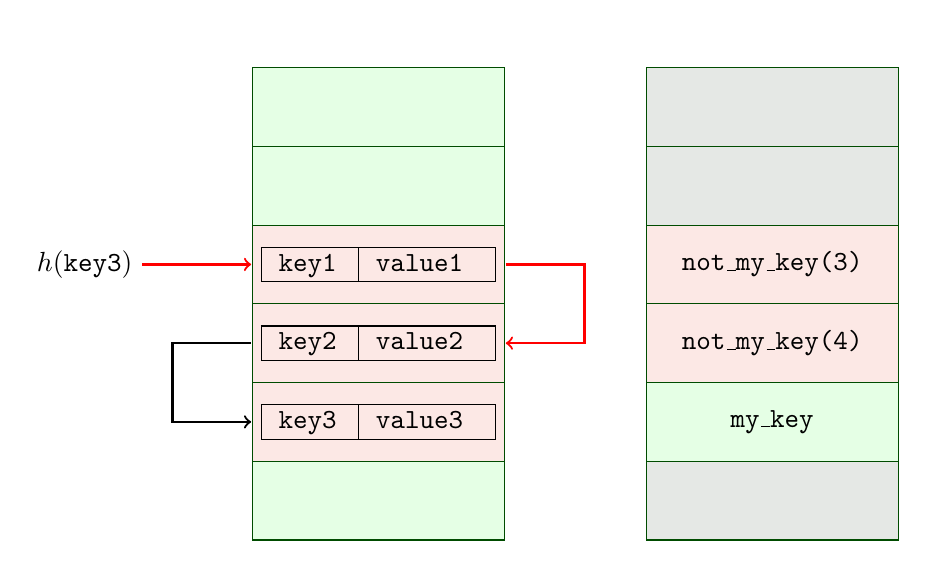
\begin{tikzpicture}
			\draw (0, -3) node[anchor=east] (key3) {$h(\mathtt{key3})$};

			\drawstruct{(8,0)}
			\structcell[padding]{} ;
			\structcell[padding]{} ;
			\structcell[occupiedcell]{\texttt{not\_my\_key(3)}} ;
			\structcell[occupiedcell]{\texttt{not\_my\_key(4)}} ; \coordinate(fourthCellOut) at (currentcell.east);
			\structcell[freecell]{\texttt{my\_key}} ;
			\structcell[padding]{} ;

			\drawstruct{(3,0)}
			\structcell[freecell]{} \coordinate(firstCell) at (currentcell.east) ;
			\structcell[freecell]{} \coordinate(secondCell) at (currentcell.east);
			\structcell[occupiedcell]{\keyvalue{key1}{value1}} \coordinate(thirdCell) at (currentcell.west); \coordinate(thirdCellOut) at (currentcell.east);
			\structcell[occupiedcell]{\keyvalue{key2}{value2}} \coordinate(fourthCell) at (currentcell.west); \coordinate(fourthCellOut) at (currentcell.east);
			\structcell[occupiedcell]{\keyvalue{key3}{value3}} \coordinate(fifthCell) at (currentcell.west); \coordinate(fifthCellOut) at (currentcell.east);
			\structcell[freecell]{} \coordinate(sixthCell) at (currentcell.east);

			\draw[->, red, thick] (key3) -- (thirdCell);
			\draw[->, red, thick] (thirdCellOut) -- ++(1, 0) |- (fourthCellOut);
			\draw[->, thick] (fourthCell) -- ++(-1, 0) |- (fifthCell);
		\end{tikzpicture}
\end{example}

In case of unsuccessful search, as in Example~\ref{expl:unsuccessful_search}, \texttt{not\_my\_key(i)} is asserted for all indexes, ensuring that the key is not present in the map.

Hence, an invariant of the \emph{for}-loop is that \texttt{not\_my\_key} is asserted \emph{for all indexes from $start$ up to $i$}, by ring accesses, $i$ being the loop iterator.

\begin{example}
	\label{expl:unsuccessful_search}
	\texttt{not\_my\_key} is ensured both when the cell is empty (green cell in this example), or when the cell is busy, but occupied by an other key (a busy cell is in red in this example).
	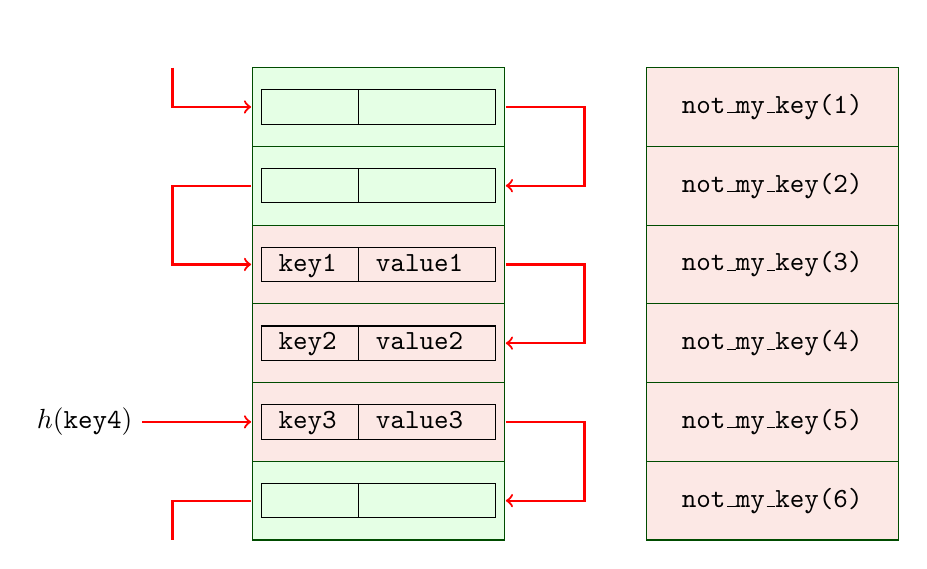
\begin{tikzpicture}
		\draw (0, -5) node[anchor=east] (key4) {$h(\mathtt{key4})$};

		\drawstruct{(8,0)}
		\structcell[occupiedcell]{\texttt{not\_my\_key(1)}} ;
		\structcell[occupiedcell]{\texttt{not\_my\_key(2)}} ;
		\structcell[occupiedcell]{\texttt{not\_my\_key(3)}} ;
		\structcell[occupiedcell]{\texttt{not\_my\_key(4)}} ;
		\structcell[occupiedcell]{\texttt{not\_my\_key(5)}} ;
		\structcell[occupiedcell]{\texttt{not\_my\_key(6)}} ;

		\drawstruct{(3,0)}
		\structcell[freecell]{\keyvalue{}{}} \coordinate(firstCell) at (currentcell.west) ; \coordinate(firstCellOut) at (currentcell.east);
		\structcell[freecell]{\keyvalue{}{}} \coordinate(secondCell) at (currentcell.west); \coordinate (secondCellOut) at (currentcell.east);
		\structcell[occupiedcell]{\keyvalue{key1}{value1}} \coordinate(thirdCell) at (currentcell.west); \coordinate(thirdCellOut) at (currentcell.east);
		\structcell[occupiedcell]{\keyvalue{key2}{value2}} \coordinate(fourthCell) at (currentcell.west); \coordinate(fourthCellOut) at (currentcell.east);
		\structcell[occupiedcell]{\keyvalue{key3}{value3}} \coordinate(fifthCell) at (currentcell.west); \coordinate(fifthCellOut) at (currentcell.east);
		\structcell[freecell]{\keyvalue{}{}} \coordinate(sixthCell) at (currentcell.west); \coordinate (sixthCellOut) at (currentcell.east);

		\draw[->, red, thick] (key4) -- (fifthCell);
		\draw[->, red, thick] (thirdCellOut) -- ++(1, 0) |- (fourthCellOut);
		\draw[->, red, thick] (fifthCellOut) -- ++ (1, 0) |- (sixthCellOut);
		\draw[red, thick] (sixthCell) -| ++(-1, -0.5);
		\draw[->, red, thick] (firstCell)+(-1, 0.5) |- (firstCell);
		\draw[->, red, thick] (firstCellOut) -- ++(1, 0) |- (secondCellOut);
		\draw[->, red, thick] (secondCell) -- ++(-1, 0) |- (thirdCell);
	\end{tikzpicture}
	
\end{example}

\begin{figure}[b]
	\lstinputlisting[language=C]{for_loop_orig_pruned.c}
	\caption{Original \emph{for}-loop for searching a key}
	\label{fig:for_loop_orig_pruned}
\end{figure}

\subsubsection{Impact of the modifications}

The modifications have two main impacts: first, the accesses are not performed in the same order. The second impact is that the specification is not true any more in the general case.

\paragraph{Access order:}
As explain above, with double hashing, cells of the map are not accessed by loop any more. Hence, the \texttt{by\_loop\_for\_all} lemma doesn't apply any more. Let $stripe$ be the function which, given a loop iteration, returns the index of the cell looked-up at this iteration (parametrized by $start$, $step$ and $capacity$). This problem is solved by computing the antecedent of each cell. 

Hence, at iteration $i$, for any cell $map[\mathtt{index}]$, if the antecedent of $map[\mathtt{index}]$ is less than $i$, then \texttt{not\_my\_key(index)} is ensured.

The new way to ensure \texttt{not\_my\_key} for all indexes is then to ensures that all index has an antecedent w.r.t. the $stripe$ function.

\paragraph{New requirements:}
However, it is not always the case that the loop eventually reach every cell. Example~\ref{expl:not_coprime} shows such a case. Actually, after the Chinese remainder theorem, the $step$ and the $capacity$ must be coprime in order to ensure that every cell is eventually tested.

Hence, this coprimeness is a new requirement of the specification. Technically, it is sufficient to have a capacity being a power of $2$ and to have only odd $offset$ hashes.

\begin{example}
	\label{expl:not_coprime}	
		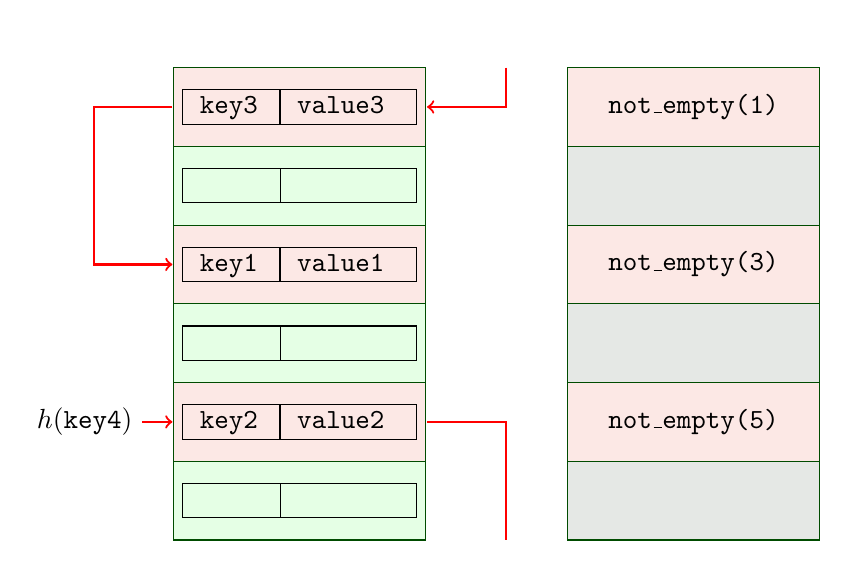
\begin{tikzpicture}
			\draw (0, -5) node[anchor=east] (key4) {$h(\mathtt{key4})$};

			\drawstruct{(7,0)}
			\structcell[occupiedcell]{\texttt{not\_empty(1)}} ;
			\structcell[padding]{} ;
			\structcell[occupiedcell]{\texttt{not\_empty(3)}} ;
			\structcell[padding]{} ;
			\structcell[occupiedcell]{\texttt{not\_empty(5)}} ;
			\structcell[padding]{} ;

			\drawstruct{(2,0)}
			\structcell[occupiedcell]{\keyvalue{key3}{value3}} \coordinate(firstCell) at (currentcell.west); \coordinate(firstCellOut) at (currentcell.east);
			\structcell[freecell]{\keyvalue{}{}} \coordinate(secondCell) at (currentcell.west); \coordinate (secondCellOut) at (currentcell.east);
			\structcell[occupiedcell]{\keyvalue{key1}{value1}} \coordinate(thirdCell) at (currentcell.west); \coordinate(thirdCellOut) at (currentcell.east);
			\structcell[freecell]{\keyvalue{}{}} \coordinate(fourthCell) at (currentcell.west); \coordinate (fourthCellOut) at (currentcell.east);
			\structcell[occupiedcell]{\keyvalue{key2}{value2}} \coordinate(fifthCell) at (currentcell.west); \coordinate(fifthCellOut) at (currentcell.east);
			\structcell[freecell]{\keyvalue{}{}} \coordinate(sixthCell) at (currentcell.west); \coordinate (sixthCellOut) at (currentcell.east);

			\draw[->, red, thick] (key4) -- (fifthCell);
			\draw[red, thick] (fifthCellOut) -| ++(1, -1.5) ;
			\draw[->, red, thick] (firstCellOut)+(1, 0.5) |-(firstCellOut);
			\draw[->, red, thick] (firstCell) -- ++(-1, 0) |- (thirdCell);

		\end{tikzpicture}
\end{example}

\subsection{The \texttt{stripe\_l\_fp} fixpoint}
\subsubsection{Definition}

First, we define a fixpoint, which returns the index to be updated after $n$ iterations with an offset of $step$, starting from $start$ with capacity $capa$. 
\marginnote{A lemma ensuring that $\mathtt{stripe} = start + n*step \% capa$ is proved.}
\begin{definition}[stripe(int start, int step, nat n, int capa)]
	\begin{lstlisting}
fixpoint int stripe(int start, int step, nat n, int capa) {
	switch(n) {
		case zero: return start;
		case succ(m): return 
			(stripe(start, step, m, capa) + step) % capa;
	}
}
	\end{lstlisting}
	
\end{definition}

The \texttt{stripe\_l\_fp} fixpoint builds a \texttt{list<option<nat>>} given a starting point, an offset, a number of accesses and a capacity. The base case of this fixpoint is to generate a \texttt{list} containing only \texttt{none}s (fixpoint \texttt{gen\_none}), if \texttt{zero} accesses are performed. The recursive case is to update the $start + n*offset \%capa$ cell, using the above \texttt{stripe} fixpoint.

\begin{definition}[stripe\_l\_fp(int start, int step, nat bound, int capa)]
	\marginnote{The \texttt{update (index, elem, list)} fixpoint returns \texttt{list} with the \texttt{index}-th element updated to \texttt{elem}.}
	\begin{lstlisting}
fixpoint list<option<nat> > stripe_l_fp(int start,
	int step, nat n, int capa)
{
	switch(n) {
		case zero: return gen_none(nat_of_int(capa));
		case succ(m): return 
			update(stripe(start, step, n, capa), some(n), 
				stripe_l_fp(start, step, m, capa));
	}
}
 	\end{lstlisting}
\end{definition}

\begin{example}[\texttt{stripe\_l\_fp(0, 2, 5, 7)}]
	Calling \texttt{stripe\_l\_fp(0, 2, 5, 7)} produces the following list. Notice that the base case returns a list containing only \texttt{none}s, not a list containing a \texttt{some(0)}. 
	\begin{center}
		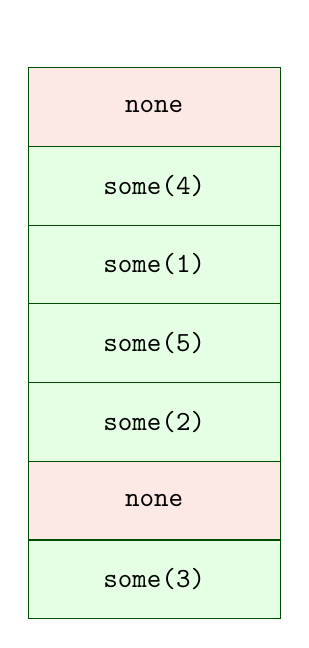
\begin{tikzpicture}
			\drawstruct{(0,0)}
			\structcell[occupiedcell]{\texttt{none}} ;
			\structcell[freecell]{\texttt{some(4)}} ;
			\structcell[freecell]{\texttt{some(1)}} ;
			\structcell[freecell]{\texttt{some(5)}} ;
			\structcell[freecell]{\texttt{some(2)}} ;
			\structcell[occupiedcell]{\texttt{none}} ;
			\structcell[freecell]{\texttt{some(3)}} ;
		\end{tikzpicture}
	\end{center}
\end{example}


\subsubsection{Properties}
The main property required is that the number of cell containing \texttt{some(i)} (for any \texttt{i}) is equal to the number of steps done. This property will later be used to ensures that the loop eventually reaches all cells (see Subsection~\ref{seq:stripe_to_stride}). The function that counts the number of such cells is named \texttt{count\_some(list<option<nat>> list)}.

There are also other properties which are used internally to prove the \texttt{count\_some} property. The main lemma is named \texttt{stripe\_l}.

\begin{lemma}[Prototype of \texttt{stripe\_l}]
	\marginnote{\texttt{list\_contains \_stripe} ensures that if a cell contains \texttt{some(i)}, then \texttt{i} is the antecedent of the cell index w.r.t. stripe.}
	\begin{lstlisting}
lemma list<option<nat> > stripe_l(int start, int step, nat n, 
	int capa)
requires 0 <= start &*& start < capa &*& step > 0 
	&*& n <= capa &*& coprime(step, capa) &*& step < capa;
ensures count_some(result) == n
	&*& length(result) == capa
	&*& true == up_to(nat_of_int(capa), 
		(list_contains_stripes)(result, start, step))
	&*& true == up_to(nat_of_int(capa), 
		(lst_opt_less_than_n)(result, n))
	&*& true == forall(result, opt_not_zero)
	&*& result == stripe_l_fp(start, step, n, capa)
	&*& coprime(step, capa);
	\end{lstlisting}
\end{lemma}

\subsubsection{Proof of \texttt{stripe\_l}}
The proof of these properties relies on the fact that the same cell is not updated twice. Once this is ensured, the construction of the fixpoint ensures the validity of the properties. 

Algorithm~\ref{alg:proof_stripe_l} shows the main steps of the proof. In the base case, all trivially holds. In the inductive case, if the \texttt{stripe(start, step, n, capa)}-th cell (i.e. the one hit at $n$-th iteration) already contains \texttt{some(i)}, the \texttt{list\_contains\_stripes} property ensures that \texttt{stripe(start, step, i, capa)}-th cell is the one we are hitting. Hence, $start + step\times i \%capa = start + step\times n \%capa$, with $n-i < capa$. Then the Chinese remainder theorem leads to a contradiction.

\begin{algorithm}
	\caption{Proof of \texttt{stripe\_l}\label{alg:proof_stripe_l}}

	\KwIn{int start, int step, nat n, int capa}	

	\Switch{n}{
		\Case{zero}{
			\tcp{All hold by construction}
		}
		\Case{succ(m)}{
			\tcp{Recursive call, the termination is ensured by n > m}
			list $lst \longleftarrow \mathtt{stripe\_l(start, step, m, capa)}$
			
			\tcp{Now, we want to update the stripe(start, step, n, capa)-th to some(n)}
			\tcp{Proof by contradiction that the cell contains none}
			\Switch{nth(stripe(start, step, n, capa), lst}{
				\Case{some(i)}{
					\Assert{$start + i\times step \%capa = start + n\times step \%capa$}\;
					\marginnote{$n-i$ is noted $diff$ in the following parts}
					\Assert{$(n-i)\times step\%capa = 0$}\;
					\Assert{$n-i < capa$}\;
					\tcp{The chinese remainder theorem applies and shows a contradiction}
					chinese\_remainder\_theorem(step, capa, $(n-i)\times step$)\;
				}
				\Case{none}{
				}
			}
			\tcp{We now that the stripe(start, step, n, capa)-th cell contains a \texttt{none}, which we update to \texttt{some(n)}, so the properties hold for the updated list.}
			\Return{update(stripe(start, step, n, capa), some(n), lst)}
			
		}
	}
\end{algorithm}

\subsubsection{From \texttt{stripe} fixpoint to \texttt{R}}
\label{seq:stripe_to_stride}

\subsection{Proof of the \emph{Chinese remainder theorem}}
\subsubsection{Properties}
The goal of the \emph{Chinese remainder theorem} is to highlight a contradiction in the \texttt{stripe\_l} proof. We have that $diff\times step\%capa = 0$. The contradiction we want to highlight is that in the given environment, $diff$ can only be $0$, i.e. the supposed previous value is the same that the one we want to write, that is the $n$-th iteration is supposed to be already written to the list.

This is reduced to the following lemma: if $x\%n1 = 0$, $x\%n2 = 0$, $n1$ and $n2$ are coprime, and $x < n1 \times n2$, then $x = 0$. It is also required that $n1 > 0$, $n2 > 0$ and $x \geq 0$.

In \texttt{stripe\_l}, this is applied to $x = diff\times \mathtt{step}$, $n1 = \mathtt{step}$ and $n2 = \mathtt{capa}$.

This lemma is a direct consequence of the \emph{uniqueness} property of the \emph{Chinese remainder theorem}. Although it is simple to show informally, Verifast first requires to build \emph{gcd} which is quite long. All the proof is done in a separate file \texttt{Chinese\_remainder\_th.gh}. 

\subsubsection{Proof by contradiction}
In Verifast, the proof of the \texttt{bin\_chinese\_remainder\_theorem} lemma is quite long (approx. 300 lines). However, most of it is only arithmetic statements. Hence, informally, the proof is much shorter. Algorithm~\ref{alg:proof_crt} sketches the main cases. The main part (\emph{if $x > 1$} branch) decomposes $x$ into $n1\times k1 = n2\times k2$. After justifying why $k1\%n2 \neq 0$, it considers $gcd(k1, n2) = a$, which can not be $1$. Then, the remaining case ($a \neq 1$, $k1\%n2 \neq 0$, $x > 1$) calls recursively the theorem, on $\frac{n2}{a} = b$.
\begin{algorithm}
	\caption{Proof of \texttt{bin\_chinese\_remainder\_theorem}\label{alg:proof_crt}}
	\uIf{$x = 1$}
	{
		$x\%n1 = 0 \Rightarrow n1 = 1$\;
		$x\%n2 = 0 \Rightarrow n2 = 1$\;
		\Assert{$n1\times n2 = 1$}\;
		\Assert{$x = n1\times n2$}\;
		\Contradiction\;
	}
	\uElseIf{$x > 1$}
	{
		$x\%n1 = 0 \Rightarrow \exists k1 | n1\times k1 = x$ \;
		$x\%n2 = 0 \Rightarrow \exists k2 | n2\times k2 = x$ \;
		\Assert{$k1 \neq 0$}\;
		\eIf{$k1\%n2 = 0$}{
			$\beta \longleftarrow k1/n2$\;
			\Assert{$\beta\times n2 = k1$}\;
			\Assert{$\beta \geq 1$}\;
			\Assert{$\beta\times n2 \leq k1$}\;
			\Assert{$x = n1\times k1 \geq n1\times n2$}\;
			\Contradiction\;
		}
		{
			$a \longleftarrow gcd(k1, n2)$\;
			$b \longleftarrow n2/a$, \Assert{$b \neq 0$}\;
			$\gamma \longleftarrow k2/a$\;
			\Assert{$gcd(b, \gamma) = 1$}\;
			\If{$gcd(n1, b) \neq 1$}{
				\Assert{$gcd(n1, a\times b) \neq 1$}\;
				\Assert{$gcd(n1, n2) \neq 1$}\;
			}
			\eIf{$a = 1$}{
				\Assert{$\gamma = k1 \wedge b = n2$}\;
				$gcd(b, \gamma) = 1 \wedge gcd(n1, b) = 1 \Rightarrow gcd(n1\times\gamma, b) = 1$\;
				\Contradiction{$gcd(x, n2) = 1$}\;
			}{
				\tcp{The termination is ensured by b < n2}
				\texttt{bin\_chinese\_remainder\_theorem}($n1$, $b$, $k2\times b$)\;
				\Assert{$k2\times b = 0$}\;
				\Assert{$k2 = 0$}\;
				\Contradiction{$n2\times k2 = x = 0$}\;
			}
		}
	}
	\Else{
		\Assert{$x = 0$}\;
	}
\end{algorithm}


\subsubsection{Assumed lemma}
One lemma remains assumed: 
\begin{lemma}[\texttt{gcd\_mul}]
	\begin{lstlisting}
lemma void gcd_mul(int n1, int n2, int n3)
requires coprime(n1, n3) &*& coprime(n2, n3);
ensures coprime(n1*n2, n3) &*& coprime(n1, n3) 
	&*& coprime(n2, n3);
	\end{lstlisting}
\end{lemma}


\section{Conclusion}
\subsection{Work done}
This semester project was two folds: 

First, analysing the provided implementation to see which part could be improved. After that, I implemented an optimization, which, I later learn, is called \emph{double hashing} (before learning that, I called it ``map with offset generator'', which explain some naming, e.g. \texttt{map\_generator.c}).

Second, formally proving the correctness of the map. The semantic of \emph{correctness} is the same as the previous one. The only difference in the specification is the requirement of coprime capacity and offset. Taking a capacity $2^n$ and an odd offset fulfils this requirement.

We completed the formal proof, except for one lemma: 
$$a\bot c \wedge b\bot c \Rightarrow (a\times b)\bot c$$
\subsection{Validity of benchmark}
We benchmarked the map to give an idea of the performance gain. Of course, performance evaluation could be much improved, with more time available. In particular, one could improve the following points: 
\begin{itemize}
	\item Test on different compilers, as GCC greater than 4.7.1 suffer from performance issues on \texttt{unordered map}.
	\item Use an other access distribution. Here, accesses are uniformly distributed. Other distribution such as Zipf's distribution might be more suitable. Another idea is to adapt some real program to this hash table to have real accesses timings.
\end{itemize}

\subsection{Forthcoming work}
Although most of the work is completed, some parts remain to do: 
\begin{itemize}
	\item The \texttt{gcd\_mul} lemma is to be proved. A way to prove it is to use the prime factor decomposition, and showing that the prime factor decomposition of a product is the union of the prime factors of two factors.
	\item Formally prove that a capacity of $2^n$ and an odd \emph{offset hash} are coprime.
\end{itemize}


\end{document}
